\chapter{Bayesian Parameter Estimation}

In classical statistics, $\mathbf\Theta$ is fixed, and the data $Y$ is generated from a distribution depending on $\mathbf\Theta$. Frequentist estimators such as the maximum likelihood estimator, or least squares estimator as previously seen are point estimates. In contrast, inference under a Bayesian framework assumes that $\mathbf\Theta$ is also a random variable. This means although inference may be done on the same model, the Bayesian statistician will more often than not end up with a probability distribution describing $\mathbf\Theta$ given $Y$.

\color{red}
\section{Monte Carlo Integration}

Let us assume we have a random variable $X\sim p,$ and we want to integrate $I = \int_{\mathcal{X}} f(x)p(x)\diff x$ with relation to some known density $p$ and function $f$. We can numerically approximate $I$ by taking $n$ i.i.d. samples $\{x_1, x_2, \dots, x_n\}$ from the distribution specified by $p$, and approximating $I$ by $I_n:=\frac{1}{N}\sum_{i = 1}^nf(x_i).$ By the strong law of large numbers, under specific conditions (for example $\sigma_f := \mathrm{Var}(f(X))<\infty$ is sufficient) we have that $I_n \to I$ almost surely as $n\to\infty$. Furthermore by the central limit theorem we know that $\sqrt{n}(I_n - I) \sim N(0, \sigma_f)$ as $n\to\infty.$ Intuitively, Monte Carlo integration works efficiently because the support set we numerically integrate over are likely to be points of higher probability density that integrating numerically over a set of uniformly distributed points.

\color{black}
\section{Accept-Reject sampling methods}

Accept-Reject methodology fundamentally relies on the theorem that $X\sim f $ is equivalent to simulating $(X,U) \sim \mathrm{Unif}\{(x, u)|0<u<f(x)\}.$ (Theorem 2.15 pg 47 Casella Roberts). In the case where a direct sampling method doesn't exist, we can use this theorem to our advantage. For example, if $a \leq X \leq b$ almost surely, then we can sample the pairs $X^*\sim \mathrm{Unif}(a, b),$ and then $U^*\sim\mathrm{Unif}(0, M),$ where $M\geq \sup_{a<x<b} f(x).$ To then get out samples to follow the distribution of $(X, U)$ we then reject all samples $(x_i, u_i)$ where $u_i>f(x_i).$ The distribution of $X$ can then be described as follows

\begin{align*}
    \Pr(X \leq x) =\,& \Pr(X^* \leq x|U^*\leq f(X^*))\\
    =\,& \frac{\Pr(X^* \leq x, U^*\leq f(X^*))}{\Pr(U^*\leq f(X^*))}\\
    =\,& \frac{\int_a^xf(y)\diff y/((b - a)*M)}{1/((b - a)*M)}\\
    =\,& \int_a^xf(y)\diff y\\
    =\,& F(x)
\end{align*}

For example in finding samples from the distribution below, we generate 100 random pairs $(X^*, U^*)$

%\begin{tikzpicture}
%\begin{axis}[axis lines = left]
%\addplot[color=red, domain = 0:1]{5*x*(x - 1)^2*(x + 2)};
%% \addplot[blue] coordinates{(\pgfmathparse{rnd}\pgfmathresult, \pgfmathparse{rnd}\pgfmathresult)};
%\end{axis}
%\end{tikzpicture}

%$\foreach \x in {1,...,10}{\pgfmathparse{rnd}\pgfmathresult, }$

There is no need for the distribution to be uniform over the rectangle, and to decrease the number of rejections we can generate points uniformly under a function $h(x)$ that more closely resembles our target distribution as long as $f(x)\leq h(x)$ for all $x$. If $h(x) = Mg(x)$ where $g(x)$ is a probability distribution function with known method of sampling, we can use this to generate via $Y\sim g$ and $U|Y\sim \mathrm{Unif}(0, Mg(x))$ then we reject all pairs where $U|Y>f(Y).$

So in the end we do\texttt{\\
1. Generate $X\sim g$\\
2. Accept if $U\leq f(X)/Mg(X)$, otherwise repeat 1.}

If $f$ is computationally expensive, but bounded below by $g_l$, we can \texttt{\\
1. Generate $X\sim g$\\
2. Accept if $U\leq g_l(X)/Mg(X)$\\
3. Accept if $U\leq f(X)/Mg(X)$, otherwise repeat 1.}

\section{Essentials for MCMC}\label{Markov_chains}

\begin{definition}[Random Walk]
    \emph{Random walk} (MCSM 6.1) is a sequence $\{X_n\}$ such that
    $$X_{n+1} = X_n + \varepsilon_n,$$ and $\varepsilon_n$ is independent from $X_1, \dots, X_n$.
\end{definition}

\begin{definition}[Transition Kernel]
    A \emph{transition kernel} is a function $K$ defined on $\mathcal{X}\times\mathcal{B}(\mathcal{X})$ such that\begin{enumerate}
    \item $\forall x\in\mathcal{X},\,\,K(x,\cdot)$ is a probability measure;
    \item $\forall A\in\mathcal{B}(\mathcal{X}),\,\, K(\cdot, A)$ is measureable.
\end{enumerate} (MCSM 6.2)
\end{definition}

\begin{definition}[Markov Chain]
    Given a transition kernel $K$, a sequence of $X_0, X_1, \dots, X_n, \dots$ of random variables is a \emph{Markov chain} denoted by $(X_n)$ if for any $t$, $$P(X_{k+1}\in A|X_0, X_1, \dots, X_k) = P(X_{k+1}\in A|X_0, \dots, X_k)$$ (MCMS 6.4)
\end{definition}

\begin{definition}[$\varphi$-irreducible]
    Given a measure $\varphi$, the Markov chain $(X_n)$ with transition kernel $K$ is \emph{$\varphi$-irreducible} if, for every $B\in\mathcal{B}(\mathcal{X})$ with $\varphi(A)>0,$ there exists $n$ s.t. $K^n(x, A)>0$ for all $x\in\mathcal{X}$. (MCSM 6.13)
\end{definition}

\begin{definition}[Atom]
    The Markov chain $(X_n)$ has an \emph{atom} ${\alpha\in\mathcal{B}(\mathcal{X})}$ if there exists an associated nonzero measure $\nu$ such that $$K(x, A) = \nu(A)$$ (MCSM 6.18)
\end{definition}

\begin{definition}[Harris Recurrent]
    A set $A$ is \emph{Harris recurrent} if $P_x(\eta_A = \infty) = 1$ for all $x\in A.$ The chain $(X_n)$ is Harris recurrent if there exists a measure $\psi$ such that $(X_n)$ is $\psi$-irreducible and for every set $A$ with $\psi(A) > 0,$ $A$ is Harris recurrent. (MCSM 6.32)
\end{definition}

\begin{definition}[Invariant (Measure)]
    A $\sigma$-finite measure $\pi$ is \emph{invariant} for the transition kernel $K(\cdot,\cdot)$ if $$\pi(B) = \int_\mathcal{X} K(x, B)\pi(\diff x), \forall B\in\mathcal{B}(\mathcal{X})$$ (MCSM 6.35) and $\pi$ is a \emph{stationary distribution} when $\pi$ is a probability measure. If such a $\pi$ exists for a $\psi$-reducible chain, the chain is \emph{positive}.
\end{definition}

\begin{definition}[Ergodic]
    For a positive Harris recurrent chain $(X_n)$, with invariant distribution $\pi$, an atom $\alpha$ is \emph{ergodic} if
    $$\lim_{n\to\infty}|K^n(\alpha, \alpha) - \pi(\alpha)| = 0$$ (MCSM 6.47)
\end{definition}

\color{black}

\section{Motivating the MH/Gibbs Algorithm}
\todo{use some of the MC theory to arrive at the acceptance probability in MH}

\section{Metropolis Hastings}

\begin{definition}[Markov Chain Monte Carlo Method]
    A \emph{Markov chain Monte Carlo method} for simulating a distribution $f$ is any method producing an ergodic Markov chain whose stationary distribution is $f$. (MCSM 7.1)
\end{definition}

Given a proposal distribution $q$, and a function $f$ proportional to the posterior distribution, the Metropolis Hastings algorithm is as follows: \texttt{\\
1. Initialise $X_0$\\
2. Generate $Y \sim q(y|x)$\\
3. Calculate $\alpha =
min\left(\frac{f(y)q(x|y)}{f(x)q(y|x)}, 1\right)$
4. $X_{t+1} = \begin{cases} Y, & \text{with probability } \alpha\\ X_{t},& \text{else}\end{cases}$
}

If $q$ is symmetric (that is $q(y|x) = q(x|y)$ for all $x, y$), then $\alpha$ simplifies down to $\frac{f(y)}{f(x)},$ and the algorithm is simply called the Metropolis algorithm.

As an example we can consider a series of coin tosses from a weighted coin. Let $p$ be the probability of a head. We assume that $p\sim\mathrm{Unif}(0,1).$ After 10 tosses \todo{when should 6 be a word}6 heads could be observed. Let $H\sim\mathrm{Binom}(10, p)$ be the number of heads that are tossed.

\begin{align*}
    \Pr(p\in\mathrm{d}p| H= 6)\propto&\, \Pr(H= 6|p\in\mathrm{d}p)\Pr(p\in\mathrm{d}p)\\
    =&\, {10 \choose 6} p^H(1 - p)^{10 - H}\\
    \propto&\, p^6(1 - p)^{4}
\end{align*}

Consider two different (symmetric) proposal distributions $q(p_i|p_{i - 1})$: \begin{itemize}
    \item $p_i^* \sim N(p_{i - 1}, 1/12)$
    \item $p_i^* \sim \mathrm{Unif}(p_{i - 1} - 1/2, p_{i - 1} + 1/2)$.
\end{itemize} Both are symmetric, and so \begin{align*}
    \alpha =&\, \min\left(\frac{f(p_i)q(p_{i - 1}|p_{i})}{f(p_{i - 1})q(p_i|p_{i - 1})}, 1\right)\\
    =&\, \min\left(\frac{{p_i}^{6}(1 - p_i)^4}{p_{i - 1}^6(1 - p_{i - 1})^4}\mathbb{I}(p_i > 0), 1\right)\\
    =&\, \min\left(\left(\frac{p_i}{p_{i - 1}}\right)^{6}\left(\frac{1 - p_i}{1 - p_{i - 1}}\right)^4\mathbb{I}(p_i > 0), 1\right)
\end{align*} The effect of the choice of proposal distribution is shown in figure \ref{fig:coin_R}.

\begin{figure}[htbp]
    \centering
    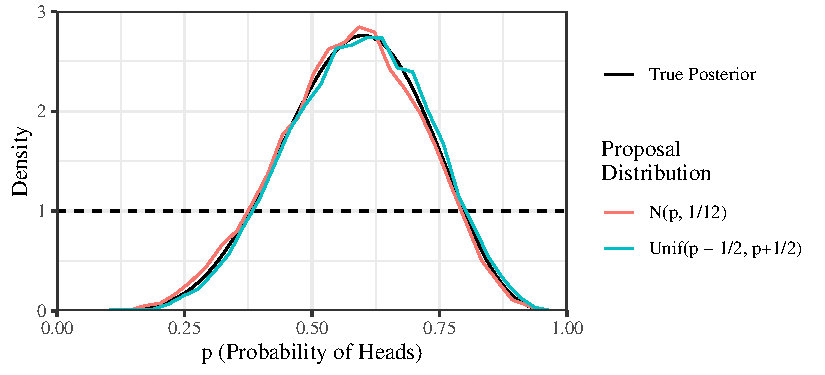
\includegraphics{coin_MH_R.pdf}
    \caption{30,000 samples from the posterior distribution of $p$ using the Metropolis Hastings algorithm. It was assumed that $p\sim \mathrm{U}(0,1)$ and $H \sim \mathrm{Binom}(10, p),$ given $H = 6.$ A uniform and normal proposal distributions were compared.}
    \label{fig:coin_R}
\end{figure}

For another example we can consider a simple SIS epidemiological model, with $$\frac{\diff S}{\diff t} = \gamma I - \beta SI \quad \frac{\diff I}{\diff t} = \beta SI -  \gamma I,$$ and a population of 25,000. Previous pandemics can be used to fix $\beta = 0.5.$ At day 0, it is assumed that there is 1 infected person. Given 1184 new cases on day 30, and $\gamma\sim \mathrm{Gamma}(2, 6)$ we can use the Metropolis Hastings algorithm to sample from the posterior distribution of $\gamma.$  This will depend on the choice of likelihood.\todo{Expand this explanation} See figure \ref{fig:SIS_MH_R}

\begin{figure}[htbp]
    \centering
    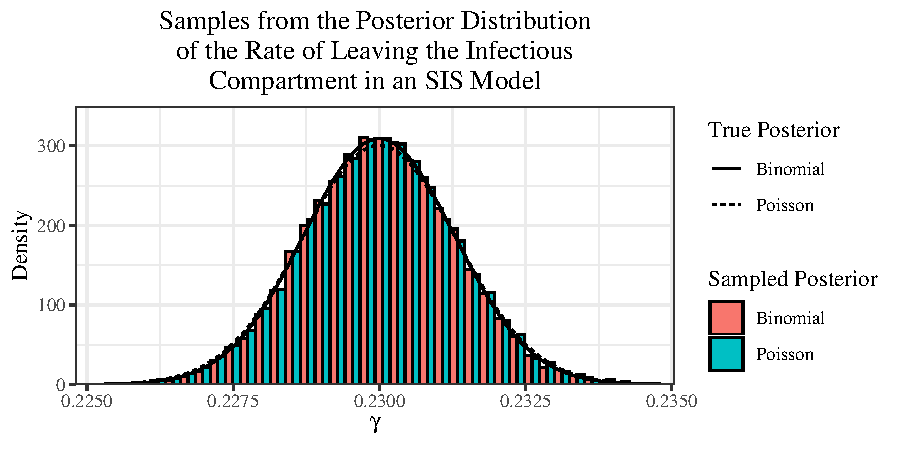
\includegraphics{SIS_gamma_pred.pdf}
    \caption{Using a basic SIS model, using incident changing likelihood function.}
    \label{fig:SIS_MH_R}
\end{figure}

\section{Gibb's Sampling}

For a multivariate case ($\mathbf{\Theta} = \{\theta_1, \theta_2, \dots, \theta_n\}$), it can be analytically or computationally intractable to calculate the posterior (or even something proportional to the posterior) distribution. In this case it may be possible to calculate $\Pr(\theta_i\in\diff\theta|\theta_1, \theta_2, \dots, \theta_{i - 1}, \theta_{i+1}, \theta_{i+2}, \dots, \theta_n, \mathrm{x})$ where $\mathrm{x}$ is the data we are fitting the parameters to.
\todo{Prove Gibbs produces sample from the posterior distribution if this is in my final paper}

In this case we can use Gibbs sampling to sample from our posterior distribution. The basic algorithm is as follows:
\texttt{\\
    Initialise for $\mathbf{\Theta} = \{\theta_1, \theta_2, \dots, \theta_n\}$\\
    1. For $i\in\{1, 2, \dots, n\}$ sample $\theta_i^* \sim \theta_i|\theta_1^*, \theta_2^*, \dots, \theta_{i-1}^*, \theta_{i+1}, \dots, \theta_n, \mathbf{x}$\\
    2. Let $\mathbf{\Theta}^* = \{\theta_1^*, \theta_2^*, \dots, \theta_n^*\}$\\
    3. Append $\mathbf{\Theta}^*$ to the chain of parameters, and let $\mathbf{\Theta} := \mathbf{\Theta}^*$
}


\begin{figure}[htbp]
    \centering
    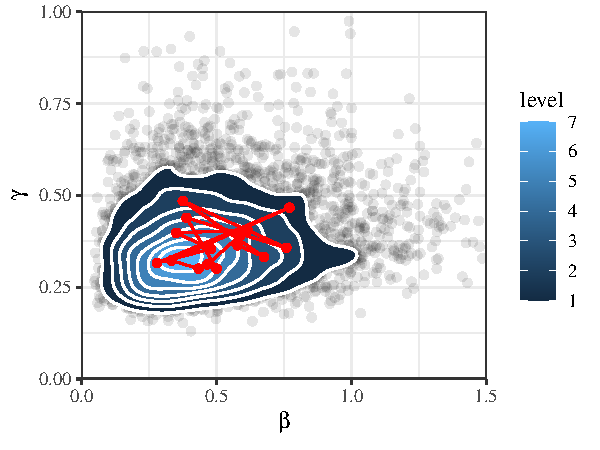
\includegraphics{SIS_gibbs.pdf}
    \caption{Using Gibbs on beta and gamma given an `$R_0$' observation}
    \label{fig:gibbs_R}
\end{figure}

\section{Diagnostics for Metropolis Hastings}
\todo{include things like autoregression, thinning, burn-in etc.}